% !TEX root=../main.tex
\documentclass[main.tex]{subfiles}

\begin{document}
\section{Abstract}
  I think therefore I am.
Neurons are the cogs of cognition.
Other important thoughts.

\section{Introduction}\label{intro_rhythms}
  % !TEX root=../main.tex

A large body of work suggests that it is difficult to write a thesis.
Yet, little is known regarding when we decided it was a good idea to do this in the first place.
If this stuff was worth knowing, wouldn't we know it already?
And still we do not.
Here, we study the effects of cognitive dissonance on the ability of researchers to study cognition \citep{Brehm:1962}.

\section{Methods}\label{intro_rhythms}
  % !TEX root=../main.tex

\subsection{Participants}
One participant was studied, the author, in an exercise of introspection. He is right-handed, 29 years old and is a solid 7. This was not approved by the IRB.

\subsection{Stimuli {\&} Task}
To engage the participant in a feeling of cognitive dissonance, we forced him to write a thesis about cognitive dissonance. The results were surprisingly effective.

\section{Results}\label{intro_rhythms}
  % !TEX root=../main.tex

We found that cognitive dissonance makes writing a thesis more difficult. No stats were used in the analysis of this finding.
\begin{figure}[H]
  \centering
  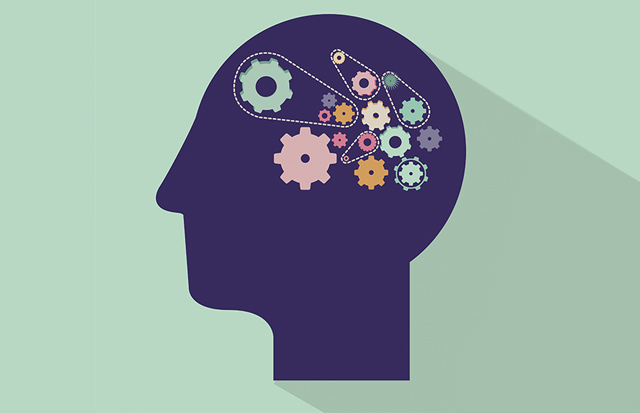
\includegraphics[width=.6\textwidth]{cognition/figures/CD.jpg}
  \caption[We're all just cogs with cogs inside of us]
  {\textit{We're all just cogs with cogs inside of us.} Here is a figure I found online \citep{CogDevUCB}.}
  \label{fig:cogsincogs}
\end{figure}

As you may see from \autoref{fig:cogsincogs}, we are mostly made up of cogs.

\section{Discussion}\label{intro_rhythms}
  Taken together, we conclude that cognitive dissonance has some effect on productivity.
Future work will analyze whether this is related to cognition or perception more directly.

% If you want a bibliography within chapter (good for sending some one a single chapter)
% make sure these lines are commented out when compiling the full thesis
% \clearpage
% \printbibliography
\end{document}
